\documentclass{article}
\usepackage[english,russian]{babel}
\usepackage[utf8]{inputenc}
\usepackage{indentfirst}
\usepackage{graphicx}
\usepackage{float}
\usepackage[margin=2cm]{geometry}

\begin{document}
\begin{titlepage}
	\begin{center}
    	ГУАП
    	\vspace{0.25cm}

    	КАФЕДРА №51
	\end{center}

    \begin{flushleft}

    	ОТЧЕТ

    	ЗАЩИЩЕН С ОЦЕНКОЙ

		ПРЕПОДАВАТЕЛЬ


    	\vspace{0.5cm}

		$\rule{5cm}{0.15mm}$ \hfill $\rule{2.2cm}{0.15mm}$  \hfill $\rule{3.25cm}{0.15mm}$

		должность, уч. степень, звание \hfill подпись, дата \hfill инициалы, фамилия
    \end{flushleft}

 	
    \hspace{2cm}

	\begin{center}
    	ОТЧЕТ ПО ЛАБОРАТОРНОЙ РАБОТЕ №11


    	\vspace{1cm}

    	ЧАТ ДЛЯ ДВУХ ПОЛЬЗОВАТЕЛЕЙ


    	\vspace{1cm}

    	по курсу: ОСНОВЫ ПРОГРАММИРОВАНИЯ {\MakeUppercase{\romannumeral 2}}
    \end{center}

    \vspace{3cm}

    \begin{flushleft}
    	РАБОТУ ВЫПОЛНИЛ

    	СТУДЕНТ ГР. № 5511 \hfill $\rule{2.2cm}{0.15mm}$  \hfill $\rule{3.25cm}{0.15mm}$

    	\hspace{7.8cm} подпись, дата \hfill инициалы, фамилия
    \end{flushleft}

	\vspace{5cm}
	\begin{center}
 		Санкт-Петербург, 2017
	\end{center}
\end{titlepage}

\section{Задание}
Написать текстовый чат для двух пользователей на сокетах. Чат должен быть реализован по принципу клиент-сервер. Один пользователь находится на сервере, второй --- на клиенте. Адреса и порты задаются через командную строку: клиенту --- куда соединяться, серверу --- на каком порту слушать. При старте программы выводится текстовое приглашение, в котором можно ввести одну из следующих команд:
\begin{itemize}
	\item задать имя пользователя (@name Vasya)

	\item послать текстовое сообщение (Hello)

	\item выход (@quit)
\end{itemize}

Принятые сообщения автоматически выводятся на экран. Программа работает по протоколу UDP.

\section{Дополнительное задание}
Добавить команды @cd, @pwd, @ls для просмотра файловой системы собеседника.
В ответ на эти команды необходимо выполнить действие с файловой системой и вернуть назад результат.

\section{Реализация}
Программа реализована двумя частями --- клиент и сервер. 

\subsection{Клиент}
За работу с клиентом отвечает класс FileSystemClient. В конструкторе получает адресс и порт для создания подключения. 
Затем в двух потоках запускаются методы client::sendMessage и client::recieveMessage, которые представляют собой бесконечные циклы, которые ожидают ввода пользователя или сообщения с сервера.\begin{itemize}
\item client::sendMessage --- отправляет сообщение, полученное из System.in, если оно не было командой @quit и @name, на сервер через DatagramSocket. 
\item client::recieveMessage --- принимает сообщения от сервера, а затем выводит их в терминал.
\end{itemize}

\subsection{Сервер}
Сервер имплементирован в классе Server. У него, так же как у клиента, есть два метода server::listener и server::respond, которые запущены в отдельных потоках. 
\begin{itemize}
\item server::respond --- отправляет сообщение, полученное из System.in, так как сервер одновременно является и клиентом.
\item client::recieveMessage --- принимает сообщения от клиента, затем проверяет, являются ли они коммандами, если нет то выводит само сообщение в терминал. 
\end{itemize}
Команды @cd, @ls и @pwd проверяются в соответствующих методах server::checkCd, server::checkLs и server::checkPwd. В них сообщение сравнивается с необходимым с помощью метода String::compareTo("command"), если они равны, то создаётся новый процесс (Process), равный выполнению данной комманды в среде выполнения программы, с помощью Runtime::exec("command"). Результат выполнения данной комманды берется из InputStream данного Process. А затем сервер отвечает клиенту с помощью метода server::respondWithMessage("message"), который отсылает необходимое сообщение через DatagramSocket.
\section{Инструкция}

\subsection{Запуск сервера}
Сервер запускается на порту указанном в 0 аргументе командной строки. Пример запуска --- java Server.java 5775.

\subsection{Запуск клиента}
При запуске клиента необходимо ввести данные адреса и порта сервера после того, как вас об этом попросят. Если все произошло успешно вы можете использовать все доступные команды. 
\\
Можно настроить имя, которое будет отображаться у собеседника, используя команду @name. Пример использования --- @name User2.
\\
Для выхода из программы нужно ввести команду @end.
\\
Для просмотра файловой системы собеседника необходимо ввести команды @ls, @cd, @pwd. 
\section{Тестирование}

\subsection{Запуск клиента}
\begin{figure}[H]
	\begin{flushleft}
		\centerline{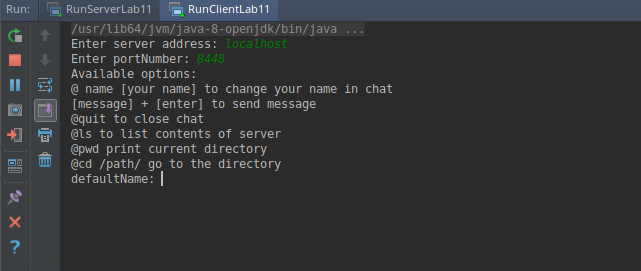
\includegraphics[scale=0.65]{clientload.png}}
		\caption{Пример запуска клиента и подключения к серверу}
	\end{flushleft}
\end{figure}

\subsection{Смена имени и отправка сообщения}
\begin{figure}[H]
	\begin{flushleft}
		\centerline{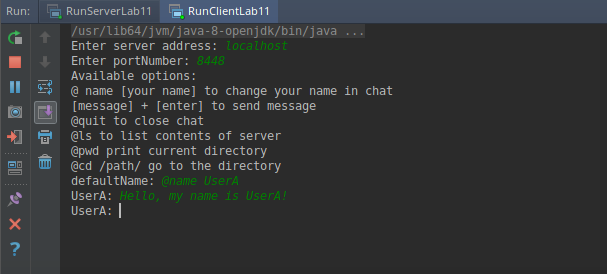
\includegraphics[scale=0.7]{nameandsend.png}}
		\caption{Смена имени командой @name и отправка сообщения на сервер}
	\end{flushleft}
\end{figure}

\begin{figure}[H]
	\begin{flushleft}
		\centerline{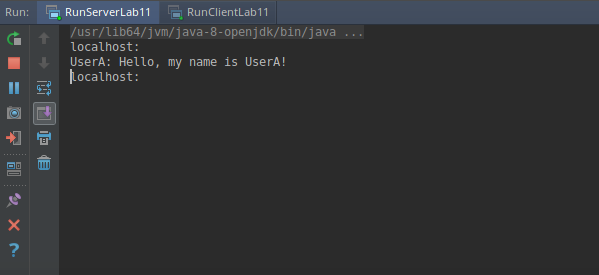
\includegraphics[scale=0.7]{servermessage.png}}
		\caption{Сообщение пришло и видно на сервере}
	\end{flushleft}
\end{figure}

\subsection{Файловая система}
\begin{figure}[H]
	\begin{flushleft}
		\centerline{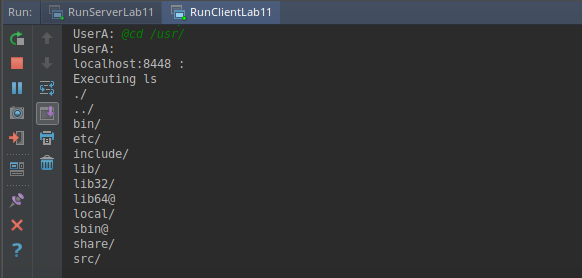
\includegraphics[scale=0.7]{cdrespond.png}}
		\caption{Введена команда @cd /usr/, сервер сменил текущую папку и прислал содержимое папки клиенту}
	\end{flushleft}
\end{figure}

\end{document}
